% By Rahul Shah
% Last Updated: Jun 23 2022, 05:28

\documentclass[11pt]{article}
\usepackage{header}
\usepackage{mathrsfs}
\usepackage{mdframed}
\usepackage{pdfpages}
\usepackage{titlesec}

\newmdenv[%
    leftmargin=-5pt,
    rightmargin=-5pt, 
    innerleftmargin=5pt,
    innerrightmargin=5pt,
    backgroundcolor=brown!10,
]{Answer}%
\def\title{Homework 01}

\def\P{\mathbb{P}} % Probability
\newcommand{\pd}[2]{\frac{\partial{#1}}{\partial{#2}}}
\let\originalmiddle=\middle
\def\middle#1{\mathrel{}\originalmiddle#1\mathrel{}}
\newcommand\aug{\fboxsep=-\fboxrule\!\!\!\fbox{\strut}\!\!\!}

\makeatletter
\newcount\my@repeat@count
\newcommand{\myrepeat}[2]{%
  \begingroup
  \my@repeat@count=\z@
  \@whilenum\my@repeat@count<#1\do{#2\advance\my@repeat@count\@ne}%
  \endgroup
}
\makeatother

\titlelabel{\thetitle.\enspace}


\begin{document}
\maketitle
\fontsize{12}{15}\selectfont

\begin{center}
    HW Due: Monday, June 27, 11:59PM
\end{center}
    
    $\textbf{Collaborators}$
    Data science is a collaborative activity. While you may talk with others about the homework, we ask that you write your solutions individually. If you do discuss the assignments with others please include their names at the top of your submission.
        \begin{Answer}
            Answer collaborators here
        \end{Answer}
        
    \textbf{
        \section*{Calculus}
    }
    \begin{enumerate}
        \item (4 points) Let $\sigma(x) = \frac{1}{1+e^{-x}}$
        \begin{enumerate}
            \item Show that $\sigma(-x) = 1 - \sigma(x)$.
                \begin{Answer}
                    Answer here
                \end{Answer}
            
            \item Show that the derivative can be written as: $$\frac{d}{dx}\sigma(x) = \sigma(x)(1 - \sigma(x))$$
                \begin{Answer}
                    Answer here
                \end{Answer}
        \end{enumerate}
    
   \newpage


    \textbf{
        \section*{Minimization}
    }
        \item (3 points) Consider the function $f(c) = \frac{1}{n}\sum_{i=1}^n (x_i - c)^2$. In this scenario, suppose that our data points $x_1, x_2, \ldots, x_n$ are fixed, and that $c$ is the only variable.\\
        Using calculus, determine the value of $c$ that minimizes $f(c)$. You must justify that this is indeed a minimum, and not a maximum.
        \begin{Answer}
            Answer here
        \end{Answer}
        
   \newpage


    \textbf{
        \section*{Probability and Statistics}
    }
        \item (2 points) Much of data analysis involves interpreting proportions – lots and lots of
        related proportions. So let’s recall the basics. It might help to start by reviewing \href{https://www.inferentialthinking.com/chapters/09/5/Finding_Probabilities.html}{\underline{the
        main rules from Data 8}}, with particular attention to what’s being multiplied in the
        multiplication rule.
        
        The Pew Research Foundation publishes the results of numerous surveys, one of which
        is about the \href{https://www.pewresearch.org/fact-tank/2019/03/22/public-confidence-in-scientists-has-remained-stable-for-decades/}{\underline{trust that Americans have}} in groups such as the military, scientists, and elected officials to act in the public interest. A table in the article summarizes the results.
        
        \ 
        
        Pick one of the options (1) or (2) to answer the question below; if you pick (1), tell us
        what $p$ is. Then, explain your choice.
        
        The percent of surveyed U.S. adults who had a great deal of confidence in both scientists
        and religious leaders
        \begin{enumerate}[1.]
            \item is equal to p\%. % comment these out selectively
            % \item \boxed{\text{is equal to } $p$\%.}
            \item cannot be found with the information in the article.
            % \item \boxed{\text{cannot be found with the information in the article.}}
        \end{enumerate}
        \begin{Answer}
            Answer here
        \end{Answer}
   \newpage
   
   
           \item (3 points) Consider the following scenario:
           
            Only 1\% of 40-year-old women who participate in a routine mammography test have breast cancer. 80\% of women who have breast cancer will test positive, but 9.6\% of women who don’t have breast cancer will also get positive tests.
            
            Suppose we know that a woman of this age tested positive in a routine screening. What is the probability that she actually has breast cancer? (Note: You must show all of your work, and also simplify your final answer to 3 decimal places.)
            \begin{Answer}
                Answer here
            \end{Answer}
    \newpage
        
        
            \item (2 points) Suppose we collected a sample of 200 students at UC Berkeley, and 150 of them happened to be Canadian (so, if we were to select a student uniformly at random from our sample, there is a 0.75 chance that they are Canadian).
            
            For inferential purposes, we choose to bootstrap this sample 500,000 times. That is, we simulate the act of re-sampling (with replacement) 200 students from our observed sample, and each time we record the number of Canadians in our re-sample.
            
            We provide a histogram of the sampling distribution below.
            \begin{figure}[h]
                \centering
                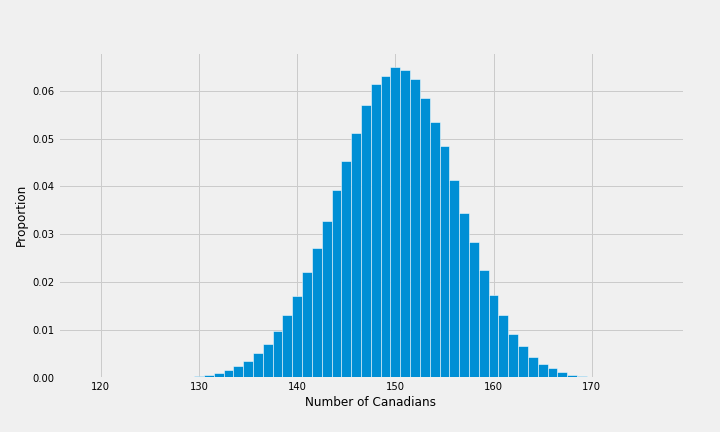
\includegraphics[scale=0.5]{histogram}
            \end{figure}
            
            What is the standard deviation of the sampling distribution shown above? Select the closest option below, and \textbf{explain your answer.}
            \begin{enumerate}[A.]
                \item 1.5
                \item 6.1
                \item 12.4
                \item 10.1
            \end{enumerate}
            \textit{Hint: While it is possible to calculate the answer, the histogram has all of the information you need.}
            \begin{Answer}
                Answer here
            \end{Answer}
   \newpage
   
   
       \textbf{
        \section*{Linear Algebra}
    }
        \item (6 points) For each part below, you will be presented with a set of vectors, and a matrix consisting of those vectors stacked in columns. State the rank of the matrix, and whether or not the matrix is full rank. If the matrix is not full rank, state a linear relationship among the vectors—for example: $\vec{v_1} = \vec{v_2}$.

        \begin{enumerate}
            \item $\vec{v}_1 = \begin{bmatrix}1\\0\end{bmatrix}, \vec{v}_2 = \begin{bmatrix}1\\1\end{bmatrix}, \ \A = \begin{bmatrix}\vert&\vert \\ \vec{v}_1&\vec{v}_2 \\ \vert&\vert \end{bmatrix}$
            \begin{Answer}
                Answer here
            \end{Answer}
            
            \item $\vec{v}_1 = \begin{bmatrix}3\\-4\end{bmatrix}, \vec{v}_2 = \begin{bmatrix}0\\0\end{bmatrix}, \ \B = \begin{bmatrix}\vert&\vert \\ \vec{v}_1&\vec{v}_2 \\ \vert&\vert \end{bmatrix}$
            \begin{Answer}
                Answer here
            \end{Answer}
            
            \item $\vec{v}_1 = \begin{bmatrix}0\\1\end{bmatrix}, \vec{v}_2 = \begin{bmatrix}5\\0 \end{bmatrix}, \vec{v}_3 = \begin{bmatrix} 10\\10 \end{bmatrix}, \ \C = \begin{bmatrix}\vert&\vert&\vert \\ \vec{v}_1&\vec{v}_2&\vec{v}_3 \\ \vert&\vert&\vert \end{bmatrix}$
            \begin{Answer}
                Answer here
            \end{Answer}
            
            \item $\vec{v}_1 = \begin{bmatrix}0\\2\\3\end{bmatrix}, \vec{v}_2 = \begin{bmatrix}-2\\-2\\5 \end{bmatrix}, \vec{v}_3 = \begin{bmatrix} 2\\4\\-2 \end{bmatrix}, \ \D = \begin{bmatrix}\vert&\vert&\vert \\ \vec{v}_1&\vec{v}_2&\vec{v}_3 \\ \vert&\vert&\vert \end{bmatrix}$
            \begin{Answer}
                Answer here
            \end{Answer}
        \end{enumerate}
    \end{enumerate}
\end{document}
